\documentclass[pdf,genome,nocolorBG,slideColor,noaccumulate,nototal]{prosper}

\usepackage{pstricks}
\usepackage{pst-grad}

\title{Cluster Workshop}

\Logo{
\includegraphics[width=.9cm]{genlogo.eps}}

\begin{document}

\begin{slide}{Cluster Workshop}
\begin{center}
	\rput(-.5,-2.75){
\includegraphics{genbanner.eps}}
\end{center}
\end{slide}

%-----------------

\begin{slide}{Introduction}
``If you were plowing a field, which would you rather use: Two strong oxen 
or 1024 chickens?''

--Seymour Cray
\end{slide}

\overlays{6}{%
\begin{slide}{Introduction}
\begin{itemstep}
	\item What is a cluster?
	\begin{itemize}
		\item A collection of machines that work together
	\end{itemize}
	\item Why use a cluster?
	\begin{itemize}
		\item Chickens are cheaper than oxen
		\item (and easier to feed)
		\item ...but try making 1024 chickens move in the same direction
	\end{itemize}
\end{itemstep}
\end{slide}}

\overlays{6}{%
\begin{slide}{Cluster Terminology}
\begin{itemstep}
	\item {\bf Core (CPU)}
	\item {\bf Hyperthreaded CPU}
	\item {\bf Socket}
	\item {\bf Core (memory)}
	\item {\bf Swap} 
	\item {\bf Thrash}
\end{itemstep}
\end{slide}}

\overlays{4}{%
\begin{slide}{Cluster Terminology}
\begin{itemstep}
	\item {\bf Node}
		An individual computer in the cluster
	\item {\bf Head Node}
		The main node.  Coordinates scheduling jobs among the nodes. 
	\item {\bf Login Node}
		The node users log in to and use to submit jobs.  May be the same
as the head node.
	\item {\bf Interconnect}
		The network or networks that connects the nodes together
	\item {\bf MPI}
		{\bf M}essage {\bf P}assing {\bf I}nterface, a protocol used for
		communication between parts of a job.
\end{itemstep}
\end{slide}}

\overlays{3}{%
\begin{slide}{Types of Jobs}
\begin{itemstep}
	\item {\bf interactive}
		A single-part job to be run immediately.
	\item {\bf batch (serial)}
		A single-part job to run in the background
	\item {\bf parallel}
		A job that has been split into multiple parts to run on more than one
		processor. 
\end{itemstep}
\end{slide}}

\overlays{3}{%
\begin{slide}{Types of Jobs}
Parallel cluster jobs can be categorized according to the amount of 
communication required between parts of the job:
\begin{itemstep}
	\item {\bf fine-grained parallel}
			Substantial communication required.
	\item {\bf course-grained parallel}
			Occasional communication required.
	\item {\bf embarrassingly parallel}
			Almost no communication required.
\end{itemstep}
\end{slide}}

\begin{slide}{Types of Jobs}

Even serial jobs that cannot be split up to run in parallel can still benefit
from a cluster environment, for example, by running with different 
sets of input files or parameters simultaneously.
\end{slide}

%-----------------

\overlays{3}{%
\begin{slide}{Cluster Storage}
\begin{itemstep}
	\item Home directory
	\item Shared cluster space
	\item Local storage
\end{itemstep}
\end{slide}}

\overlays{3}{%
\begin{slide}{Storage: Home directory}
\begin{itemstep}
	\item Network mounted
	\item Geared towards wide availability, not high performance
	\item Good place for your code, final results
\end{itemstep}
\end{slide}}

\overlays{4}{%
\begin{slide}{Storage: shared}
\begin{itemstep}
	\item Network shared, but only within the cluster
	\item Medium availability, medium performance
	\item Good place for dataset that all nodes need to access
	\item Performance can suffer with many simultaneous accesses
\end{itemstep}
\end{slide}}

\overlays{3}{%
\begin{slide}{Storage: local}
\begin{itemstep}
	\item Not network shared, only available to a single node
	\item Highest performance, but least convenient
	\item Good place for working set
\end{itemstep}
\end{slide}}

\begin{slide}{Anatomy of a Cluster}
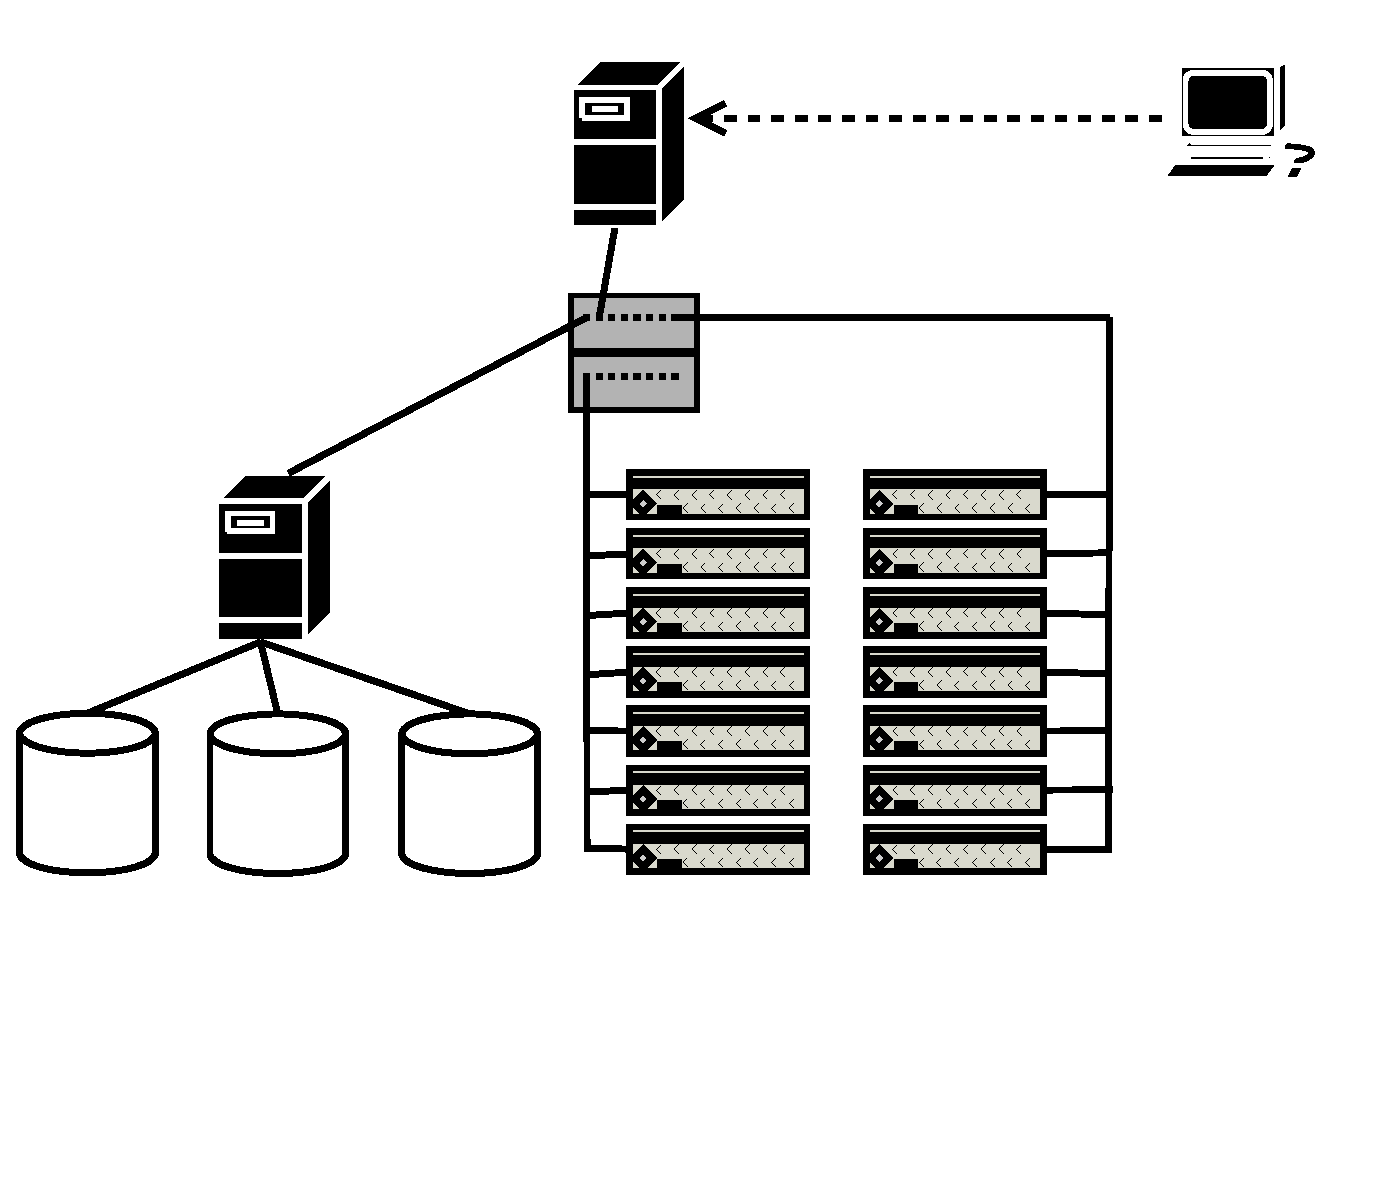
\includegraphics[height=8cm]{cluster_network.eps}
\end{slide}

\overlays{6}{%
\begin{slide}{Sun Grid Engine}
\begin{itemstep}
	\item What is a batch queue?
	\begin{itemize}
		\item Manage cluster resources
	\end{itemize}
	\item Why use the batch queue?
	\begin{itemize}
		\item Share cluster resources
		\item You don't need to worry about when/where your jobs run
		\item Submit a whole bunch of jobs and go home!
	\end{itemize}
\end{itemstep}
\end{slide}}

\overlays{3}{%
\begin{slide}{The Cluster Caf\'{e} }
You can think of the cluster as a restaurant:
\begin{itemstep}
	\item {\bf Jobs} are parties coming to eat
	\item {\bf Tables} are the nodes of the cluster
	\item Usually the scheduler will try to place each job at its own table,
		but if it's a busy day, you might have to share a table with someone
		you don't know.
\end{itemstep}
\end{slide}}

\overlays{4}{%
\begin{slide}{Slots}
A {\bf slot} is a placeholder where a job or part of a job can run.  In
the Cluster Caf\'{e}, it is a chair at a table.
\begin{itemstep}
	\item A resource allocated to your job.
	\item We define one slot per CPU core
	\item Request number of slots when you submit job
	\item Allocating a slot is only advisory: the scheduler has reserved
		the requested number of slots.
\end{itemstep}
\end{slide}}

\overlays{5}{%
\begin{slide}{Resources}
\fromSlide{1}{%
It is possible to request other resources when you submit your job}

\fromSlide{2}{%
\hskip 1cm $\Rightarrow$``I'd like a table by the window''}
\vskip .5cm
\fromSlide{3}{%
Or even to request a specific node}

\fromSlide{4}{%
\hskip 1cm $\Rightarrow$``I want to sit at table 2. I'll wait.''}
\vskip .5cm
\fromSlide{5}{%
The scheduler will wait to run your job until it can fulfill your
requirements.}
\end{slide}}

\overlays{3}{%
\begin{slide}{Parallel Environment}
A {\bf Parallel Environment} sets up the resources required to run a multi-node
job. 
\begin{itemstep}
	\item Need to use a PE when you want more than one slot
	\item Request desired PE when you submit your job
\end{itemstep}
\fromSlide{3}{%
Tells the scheduler how you'd like the table set}
\end{slide}}

\overlays{2}{%
\begin{slide}{Parallel Environment}
\begin{itemstep}
	\item mpi
		Sets up environment for distributed jobs using MPI
	\item serial/threaded
		Makes sure all slots are on the same node, does not set up any inter-node
		communication environment.
\end{itemstep}
\end{slide}}

\overlays{3}{%
\begin{slide}{Task Arrays}
\begin{itemstep}
	\item Run the same job multiple times
	\item submit/manage as a single job
	\item Ideal for running the same program repeatedly with different
         input files or parameters
\end{itemstep}
\end{slide}}

\overlays{2}{%
\begin{slide}{Resources}
Resources represent the hardware and software configuration of a node.
They can represent things like memory, CPU architecture, or software
licenses.

They come in two basic flavors:
\begin{itemstep}
	\item {\bf non-consumable} - they don't go away when requested
	\item {\bf consumable} - when requested, the resource is marked as
used until the job requesting them is finished.
\end{itemstep}
\end{slide}}

\overlays{6}{%
\begin{slide}{SGE Commands}
\begin{itemstep}
	\item qsub/qlogin/qsh: submit jobs
	\item qstat: get job status
	\item qdel: remove a job
	\item qlogin: interactive login
	\item qalter: change a job after submission
	\item qacct: view accounting information
\end{itemstep}
\end{slide}}

\overlays{3}{%
\begin{slide}{Job submission}
\begin{itemstep}
	\item {\bf qsub} - submit your job in the background
	\item {\bf qlogin} - interactive login
	\item {\bf qsh} - interactive login with X
\end{itemstep}
\end{slide}}

\overlays{3}{%
\begin{slide}{Things to do}
\begin{itemstep}
	\item Use the scheduler!
	\item Checkpoint your job
	\item Make use of local storage on the nodes for intermediate results
\end{itemstep}
\end{slide}}

\overlays{3}{%
\begin{slide}{Things NOT to do}
\begin{itemstep}
	\item Run jobs on the head node
	\item Many simultaneous writes to network filesystem
	\item Go around scheduler and run directly on the nodes
\end{itemstep}
\end{slide}}

\end{document}
